% \iffalse
\documentclass[journal,12pt,twocolumn]{IEEEtran}
\usepackage{amsmath,amssymb,amsfonts,amsthm}
\usepackage{txfonts}
\usepackage{tkz-euclide} 
\usepackage{listings}
\usepackage{gvv}       
\usepackage[latin1]{inputenc}   
\usepackage{array}  
\usepackage{tikz}
\usepackage{circuitikz}

\begin{document}

\bibliographystyle{IEEEtran}

\vspace{3cm}

\title{}
\author{EE23BTECH11217 - Prajwal M$^{*}$
}
\maketitle
\newpage
\bigskip

\renewcommand{\thefigure}{\theenumi}
\renewcommand{\thetable}{\theenumi}

\section*{Exercise 9.1}
The given figure shows a series LCR circuit connected to a sinusoidal 230 V source. \\
L = 5.0 H, C = 80 $\mu$F, R = 40 $\Omega$.

\begin{figure}[h]
\begin{center}
\begin{circuitikz}[american voltages]
      \draw (0,0)
      to[sV, l=$\varepsilon$] (0,2)
      to[R, l=$R$] (4,2)
      to[C, l=$C$] (4,0)
      to[L, l=$L$] (0,0);
\end{circuitikz}
\end{center}
\label{217.fig.1}

\end{figure}

\begin{enumerate}
    \item Determine the source frequency which drives the circuit in resonance.
    \item Obtain the impedance of the circuit
at the resonating frequency.
    \item Determine the rms potential drops across the three elements of
the circuit. Show that the potential drop across the LC
combination is zero at the resonating frequency.\\
\end{enumerate}

Solution:
\begin{table}[h]
    \centering
    \begin{tabular}{|c|c|c|}
\hline
\textbf{Paramater} & \textbf{Description} & \textbf{Value}  \\ \hline
$V\brak{t}$ & Voltage power supply & $230\sqrt{2} cos\brak{2\pi f t}$ V  \\ \hline
$V\brak{s}$ & Laplace transform of $V\brak{t}$ & ? \\\hline
L & Inductance & $5.0$ H  \\ \hline
C & Capacitance & $80\,\mu$F \\ \hline
R & Resistance & $40\,\Omega$ \\ \hline
$f$ & Frequency of voltage source & ? \\ \hline 
$Z$ & Impedance of circuit & ? \\ \hline
$V_R\brak{t}$ & Potential drop across Resistor & ?\\ \hline
$V_R\brak{s}$ & Laplace transform of $V_R\brak{s}$ & ?\\\hline
$V_C\brak{t}$ & Potential drop across Capacitor & ?\\ \hline
$V_C\brak{s}$ & Laplace transform of $V_C\brak{s}$ & ?\\\hline
$V_L\brak{t}$ & Potential drop across Inductor & ?\\ \hline
$V_L\brak{s}$ & Laplace transform of $V_L\brak{s}$ & ?\\\hline
\end{tabular}

    \caption{Parameter description}
    \label{tab:217.tab.1}
\end{table}
\begin{figure}[h]
	\begin{center}
\begin{circuitikz}[american voltages]
      \draw (0,0)
      to[sV, l=$\varepsilon$] (0,2) 
      to[R, l=$R$, v=$V_R$, i=$I$] (4,2) 
      to[R, l=$\frac{-j}{\omega C}$, v=$V_C$] (4,0)
      to[R, l=$j\omega L$, v=$V_L$] (0,0);
\end{circuitikz}
\caption{circuit diagram}
\label{217.fig.2}
\end{center}

\end{figure}

\begin{enumerate}
\item 
from \figref{217.fig.2},
\begin{align}
    Z & = R + j\brak{\omega L - \frac{1}{\omega C}}\\
    min\brak{|Z|} & = R \text{ at } \omega = \frac{1}{\sqrt{LC}}\\ 
    f_{res} = \frac{\omega_{res}}{2\pi} & = \frac{1}{2\pi\sqrt{LC}} = 7.958 Hz \label{217.eq.3}
\end{align}
\item 
\begin{align}
    Z_{res} & = R = 40 \Omega\label{217.eq.4}
\end{align}

\begin{figure}[h]
     \centering
	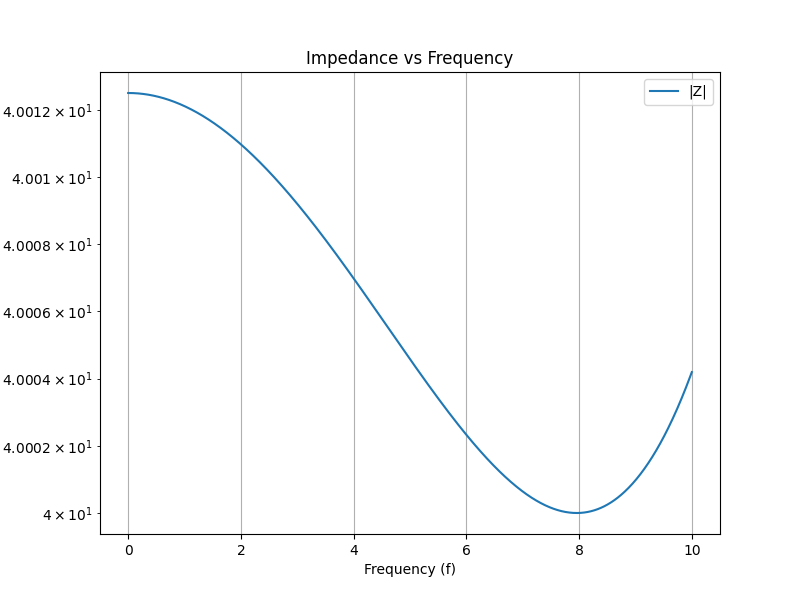
\includegraphics[width=\columnwidth]{figs/impedance.png}
     \caption{Impedance vs frequency}
     \label{217.fig.3}
\end{figure}

\item 
\begin{align}
    I_{res} & = \frac{\varepsilon}{Z_{res}}\label{217.eq.5}\\
    % & = \brak{\frac{230\sqrt{2}e^{j\omega_{res}t}}{R}}\\
    % I_{res} & = \brak{8.132}e^{j50t}\label{217.eq.5}\\
    V_R & = Re\cbrak{RI_{res}}\\
    & = Re\cbrak{R\frac{\varepsilon}{Z_{res}}}&\cbrak{\text{using \eqref{217.eq.5}}}\\
    & = Re\cbrak{325.28e^{j50t}}\\
    & = 325.28 cos\brak{50t}\\
    V_C & = Re\cbrak{\frac{-j}{\omega_{res}C}I_{res}}\\
    & = Re\cbrak{\frac{-j}{\omega_{res}C}\frac{\varepsilon}{Z_{res}}}&\cbrak{\text{using \eqref{217.eq.5}}}\\
    & = Re\cbrak{2032.93 e^{j\brak{50t - \frac{\pi}{2}}}}\\
    & = 2031.93 sin\brak{50t} \label{217.eq.7}\\
    V_L& = Re\cbrak{j\omega_{res}LI_{res}}\\
    & = Re\cbrak{j\omega_{res}L\frac{\varepsilon}{Z_{res}}}&\cbrak{\text{using \eqref{217.eq.5}}}\\
    & = Re\cbrak{2032.93e^{j\brak{50t + \frac{\pi}{2}}}}\\
    & = - 2031.93 sin\brak{50t} \label{217.eq.8}
\end{align}

from \eqref{217.eq.7} and \eqref{217.eq.8}, voltage across LC combination is $V_C + V_L = 0 V$
\end{enumerate}

\begin{table}[h]
    \centering
    \begin{tabular}{|c|c|c|}
\hline
\textbf{Paramater} & \textbf{Description} & \textbf{Value}  \\ \hline
$f_{res}$ & resonant source frequency & $7.958 Hz$\\\hline
$Z_{res}$ & resonant impedance & $40 \Omega$\\\hline
$V_{R}$ & rms value of $V_R \brak{t}$ & $230 V$\\\hline
$V_{C}$ & rms value of $V_C \brak{t}$ & $1437.5 V$\\\hline
$V_{L}$ & rms value of $V_L \brak{t}$ & $14375 V$\\\hline
\end{tabular}

    \caption{Solution values}
    \label{tab:217.tab.2}
\end{table}

\begin{figure}[h]
     \centering
	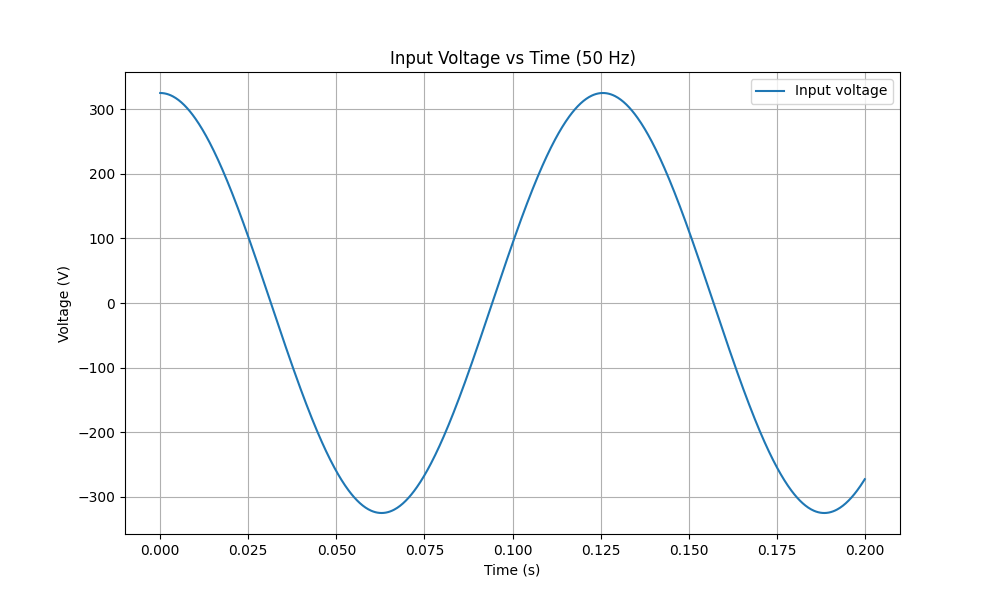
\includegraphics[width=\columnwidth]{figs/Vin.png}
     \caption{Input voltage}
     \label{217.fig.5}
\end{figure}

\begin{figure}[h]
     \centering
     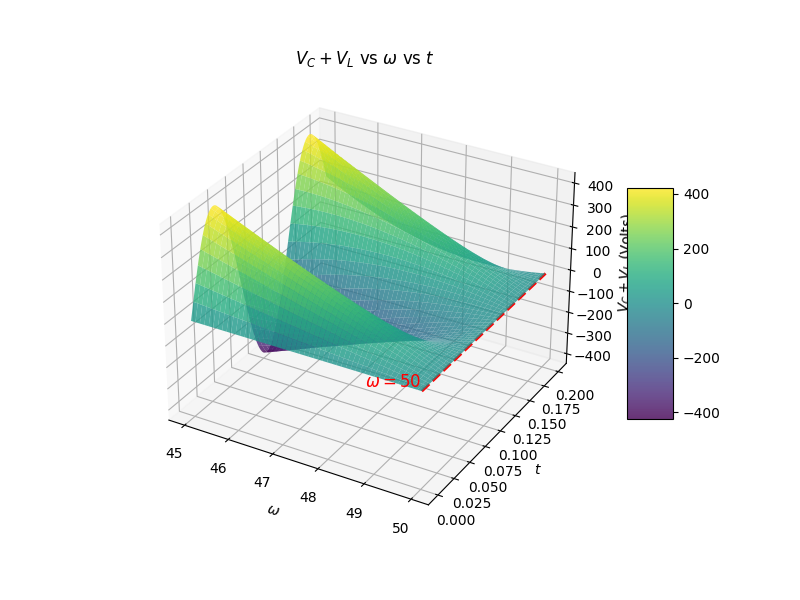
\includegraphics[width=\columnwidth]{figs/LCvoltage.png}
     \caption{Voltage across LC combination}
     \label{217.fig.4}
\end{figure}
\end{document}
